\documentclass[10pt,twocolumn]{article}

\usepackage{times}
\usepackage{mathptmx}  
\usepackage{spverbatim}
\usepackage{fixltx2e}
\usepackage[utf8]{inputenc}
\usepackage{graphicx}
\usepackage{sidecap}
\usepackage{fancyhdr}
\usepackage{amssymb,amsmath}
\usepackage[swedish]{babel}
\usepackage[margin=1.5in]{geometry}
\usepackage{abstract}
\usepackage[parfill]{parskip}
\usepackage{tocloft}
\usepackage{adjustbox}
\usepackage{textcomp}
\usepackage[T1]{fontenc}
\usepackage{listings}
\usepackage{xcolor,colortbl}
\usepackage{hyperref}
\usepackage{mcode}
\usepackage{a4wide}
\usepackage{caption}
\usepackage{epstopdf}
\usepackage{pdfpages}

\raggedbottom
\sloppy

\title{Laborationsrapport i TSKS10 \emph{Signaler, Information och Kommunikation}}

\author{Hans-Filip Elo, hanel742, 900109-5174}

\begin{document}

\maketitle

\section{Syfte}

Syftet med denna laboration är att finna bärfrekvens för en given signal, filtrera bort oönskade delar av överföringen och sedan I-/Q-demodulera signalen för att extrahera relevant information. 

\section{Materiel och förutsättningar}

Filen signal-hanel742.wav är given med den kända samplingsfrekvensen 400 kHz. Givet är också att filen innehåller en smalbandig signal som är I-/Q-modulerad och har skickats genom filtret nedan. 

\begin{gather}
h(t) = \delta(t - \tau_1) + \delta(t - \tau_2)
\label{equ:filter}
\end{gather}

På förhand ges också att bärfrekvensen för relevant del av signalen är en multipel av 19 kHz.

Signalen innehåller två melodier, två olika ordspråk samt vitt brus. 

För att utföra laborationen används GNU Octave med vertygslådor för ljud samt signaler (octave-audio och octave-signal) installerat. 

% -------- Metod ------------
\section{Metod}

Jag börjar med att läsa in filen i Octave och sedan fouriertransformera signalen för att få ut dess frekvensspektrum: 

\begin{figure}[htp]
  \begin{center}
  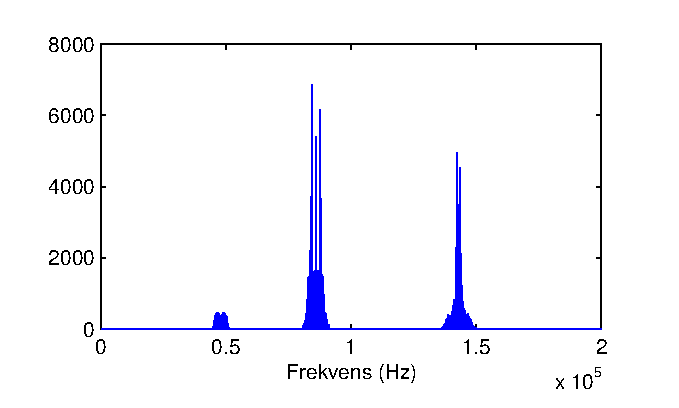
\includegraphics[keepaspectratio=true,width=\linewidth]{fft_orig_data_oneside.eps}  %skala och filnamn. 
  \end{center}
  \caption{Enkelsidigt amplitudspektrum för ursprunglig signal} %figurtext.
  \label{fig:fft_orig_data}
\end{figure}

\subsection{Att finna bärfrekvensen}

Jag vill nu filtrera ut signalelementen för de olika topparna ur totala signalen. 

Genom att utläsa frekvenserna ur topparna i figur~\ref{fig:fft_orig_data} kan man se att topparna har bärfrekvenser i området kring frekvenserna $4,959 \cdot 10^4$, $8,313 \cdot 10^4$ samt $1,412 \cdot 10^5$.

Filtrerar man sedan den givna signalen med hjälp av bandpassfilter kring dessa frekvenser och plottar graferna kan man sedan genom att studera graferna uppskatta vilken information respektive frekvensband innehåller. . 

\begin{figure}[htp]
  \begin{center}
  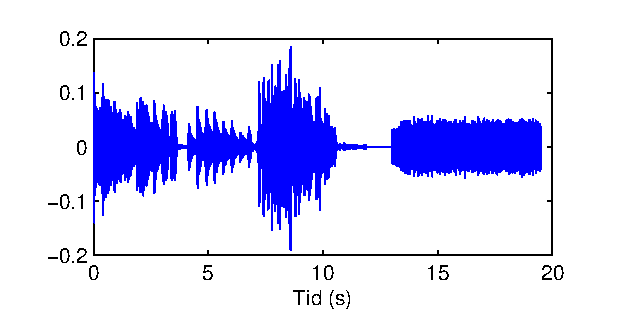
\includegraphics[keepaspectratio=true,width=\linewidth]{topp1.eps}  %skala och filnamn. 
  \end{center}
  \caption{Frekvenstopp 1 filtrerad} %figurtext.
  \label{fig:topp1_filter}
\end{figure}

Enligt utseendet på graferna ser frekvenstopp i figur~\ref{fig:topp1_filter} ut att innehålla två intervall med någon form av information, följt av brus mot slutet. Detta är precis det utseende vi eftersöker enligt given uppgift. 

Närmsta multipel av 19 kHz för den uppskattade bärfrekvensen, $f_c$, för frekvenstoppen i figur~\ref{fig:topp1_filter} är 57 kHz, vilket väljs till bärfrekvens för fortsatta experiment. 

\subsection{Filtrering}

När signalen skickas genom filtret givet i uppgiften skapas ett eko med styrkan $90\%$ av ursprungliga signalen. Detta eko har en tidsfördröjning som är lika med beloppet av differensen av filtrets två tidsfördröjningar, alltså $|\tau_1 - \tau_2|$.

Fördröjningen ges relativt enkelt ur mångtydighetsfunktionen\footnote{Signals, Information and Communications, kapitel 4, Larsson Erik G, draft 11342, februari 2014} för det vita bruset som finns i slutet av vår filtrerade signal. Jag använder det vita bruset då detta är helt okorrelerat. Detta ger tre tydliga toppar i grafen. Tidsfördröjningen kan sedan utläsas som differensen mellan två intilliggande toppars position. I figur \ref{fig:xCorr} syns två toppar.  
\begin{figure}[htp]
  \begin{center}
  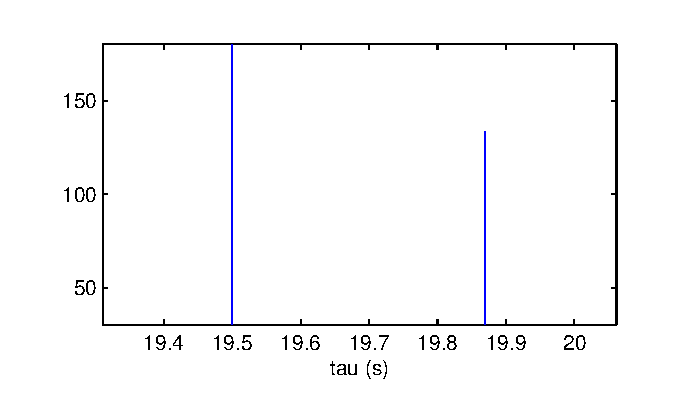
\includegraphics[keepaspectratio=true,width=\linewidth]{xCorr.eps}  %skala och filnamn. 
  \end{center}
  \caption{Mångtydighetsfunktion för vitt brus} %figurtext.
  \label{fig:xCorr}
\end{figure}
Mätningar ur figur \ref{fig:xCorr} ger att tidsfördröjningen är lika med $370\;ms$. 

Då vi samplar med en frekvens av $400 000\;Hz$ ges tidsfördröjningen $|\tau_1 - \tau_2|$ i antal samples (n) enligt nedan 

\begin{gather}
n = 0,370 \cdot 400 000 = 148 000
\label{equ:delaySamples}
\end{gather}
Innan man kan I-/Q-demodulera signalen behöver det eko som uppstår då signalen passerar det givna filtret tas bort. 

De första $n$ antal samples innehåller inget eko. Nästkommande $n$ samples innehåller eko som kan tvättas bort med förstkommande $n$ samples. När $n+n$ samplingar är fria från eko kan man använda samplingar $n-(2n-1)$ för att tvätta bort eko från nästkommande $n$ samples. Processen upprepas tills dess att hela signalen är fri från eko. Ett steg i processen utförs alltså enligt nedan

\begin{gather}
S_{utan eko}^{aktuell} = S_{eko}^{aktuell} - 0,9S_{utan eko}^{tidigare}
\label{equ:eko}
\end{gather}

Där $S_{utan eko}^{aktuell}$ är aktuella samples utan eko, $S_{eko}^{aktuell}$ de just nu aktuella samplingarna som tvättas, och $S_{utan eko}^{tidigare}$ är de förekommande $n$ samplingarna. 

\subsection{I-/Q-demodulation}

För att demodulera signalen används principer som beskrivs av Erik G. Larsson (2014). I- och Q-komponenter ges enligt nedan: 

\begin{gather}
x_{I}(t) = \Large{H}_{B/2\;Hz}^{LP}\{2x(t)\cos{(2{\pi}f_{c}t + \theta)}\} \\
x_{Q}(t) = -\Large{H}_{B/2\;Hz}^{LP}\{2x(t)\sin{(2{\pi}f_{c}t + \theta)}\}
\label{equ:iq}
\end{gather}

Där $\theta$ är fasförskjutningen, $x(t)$ signalen som demoduleras, $B$ bandbredden hos signalen vid den ursprungliga samplingen av den, samt att $x_{I}(t)$ och $x_{Q}(t)$ är de demodulerade signalbanden. 

Signalerna demoduleras först. Fasförskjutningen testats sedan fram genom att lyssna på resulterande ljudet av signalen. Fasföskjutningen kan vara vilken vinkel som helst. Då $sin(\theta)$ blir $cos(\theta)$ efter $\frac{\pi}{2}$ och vise versa. 

Fasförskjutningen för signalen testades fram till $0$


% -------- Slutsatser ------------
\section{Resultat och slutsats}

Funna egenskaper hos signalen är: 

\begin{itemize}
	\item $f_c = 57$ kHz
	\item $|\tau_1 - \tau_2| = 370$ ms
  \item Fasföskjutningen, $\theta = 0$
\end{itemize}

Först spelas två melodier - varav en blinka lilla stjärna. Sedan hörs två ordsspråk. Ordspråken som hörs är: 

\begin{itemize}
	\item ''Man kan inte både ha kakan och äta den''
	\item ''Man ska inte säga Hin i död mans hus''
\end{itemize}
% -------- Appendix ---------------

\includepdf[pages={-}]{appendix.pdf}

\end{document}